% Chapter 2
\chapter{Background}\label{ch:background} % For referencing the chapter elsewhere, use \autoref{ch:examples} 
\minitoc% Creating an actual minitoc\
\bigskip

In this chapter, we describe the main concepts and principles behind system dependability, observability in distributed systems, and the use of artificial intelligence in IT operations (AIOps). Then, we explain key concepts of anomaly detection needed for understanding the methods in this thesis. 

\section{System Dependability}
Dependability is defined as the trustworthiness of a computer system such that reliance can justifiably be placed on the service it delivers~\cite{carter1982time}. In software engineering, dependability can be broken down into three elements~\cite{Laprie1992}:
\begin{enumerate}
    \item The threats (impairments) to dependability: faults, errors, failures; they are
undesired circumstances causing that reliance cannot, or will not longer be placed on the service.
    \item The means for dependability: fault prevention, fault tolerance, fault
removal, and fault forecasting, which provide the ability to deliver a service on which
reliance can be placed.
    \item The attributes of dependability: Depending on the application running in the system, dependability may be viewed according to different, but complementary, properties: (1) with respect to the readiness for usage, dependable means available; (2) with respect to the continuity of service, dependable means reliable; (3) with respect to the avoidance of catastrophic consequences on the environment, dependable means safe; and (4) with respect to the prevention of unauthorized access and/or handling of information, dependable means secure~\cite{Laprie1992}. 
\end{enumerate}

The methods presented in this theses are contributing towards the improvement of dependability of the distributed systems by detecting the threats to system dependability. In the following we describe the concepts behind faults, errors, and failures.

A \textbf{fault} or bug is a defect in a system. The presence of a fault in a system may or may not lead to a failure. For example, although a system may contain a fault, its input and state conditions may never cause this fault to be executed so that an error occurs. 

An \textbf{error} is a difference between the desired behaviour of a system and its actual behaviour. Errors usually occur at runtime when some part of the system enters an unexpected state due to the activation of a fault. Since errors are generated from invalid states they are hard to observe without special mechanisms, such as debuggers or debug output to logs.

A \textbf{failure} is an instance in time when a system displays behaviour that is contrary to its specification. An error may not necessarily cause a failure, for instance an exception may be thrown by a system but this may be caught and handled using fault tolerance techniques so the overall operation of the system will conform to the specification.

In modern paradigms of distributed software systems, ensuring high dependability is a challenging problem as the threats can appear in hardware failures, unreliable networks, software bugs, and even human errors~\cite{imweber2015}. In the following, we describe key concepts of distributed systems, and observability as a key paradigm that provides the starting point for improving the dependability.

\section{Distributed system observability}
\label{ch:background:sec:observability}
A distributed system has multiple components located on different machines, which communicate and coordinate actions over the network by passing messages to each other~\cite{tanenbaum2007distributed}.
SOAs have been introduced more than 20 years ago~\cite{abrams2008service}. Since then, the field of distributed systems has been actively researched, which has led to a large paradigm shift. Recently, a variant of SOA, referred to as microservice architecture, emerged as a standard architecture for software systems. Today, more than two decades after the introduction of SOA, systems based on microservices are state of the art and utilized by major companies such as Google, Twitter, and Amazon~\cite{observability2020practical}. Furthermore, cloud providers such as Amazon Web Services and Microsoft Azure enabled companies to migrate their infrastructures into the cloud, where ideas similar to microservices can be easily implemented. This facilitated the general paradigm shift in software~\cite{jungnickel2018feasibility}. 

The conceptual change in software architectures implies that the services increasingly rely on communication. This introduces an additional complexity into the distributed systems. The increased complexity of a highly distributed architecture leads to difficulties in O\&M, which directly affects the reliability, availability, resilience, and security of the systems~\cite{newman2015building}.
Availability is a characteristic of a system, which aims to ensure an agreed level of operational performance, usually uptime, for a higher-than-normal period. Reliability is the probability of continuous correct operation~\cite{malkawi2013art}.

Owing to the complexity, distributed systems are prone to failures and are not available at all times at 100\%~\cite{gunawi2014bugs,sillito2020failures}. Building dependable with respect to reliability systems requires context-aware monitoring of the distributed infrastructure, which is referred to as observability. Therefore, collecting every possible snapshot of the system can be used to develop intelligent tools to support troubleshooting and operations such as anomaly detection, root-cause analysis, and probably self-healing triggers into the system~\cite{observability2020practical}. 

Observable systems require the collection of factual data and extraction of insightful information. The distributed system data are in the forms of metrics, logs, and traces, often referred to as three pillars of observability~\cite{nedelkoski2020data,observability2020practical}.
Metrics are numeric values measured over a period of time. They describe the utilization and status of the infrastructure, typically regarding the CPU, memory, disk, network throughput, service latency, and error rates~\cite{nedelkoski2019anomaly,schmidt2018iftm,}. 
Logs enable developers to record actions executed at runtime by software. Services and other systems generate logs composed of timestamped records with a structure and free-form text~\cite{jakublogs,tang2011logsig,du2017deeplog,meng2019loganomaly}.
Distributed traces record the workflows of services executed in response to requests, e.g., hypertext transfer protocol (HTTP) or remote procedure call (RPC) requests. The records contain information about the execution graph and performance at a microservice level~\cite{RepTrace,nedelkoski2020selftracing,nedelkoski2019anomalymultimodal}.

Notably, these major observability components can be instrumented and available for most distributed software system, as they comply with modern software engineering practices~\cite{sridharan2018distributed}. 
We describe each of the system data sources below.

\subsection{Metrics}\label{ch:background:sec:observability:subsec:metrics}
Most components of the software infrastructure serve as a resource to other components or systems. Some resources are low-level, e.g., server resources such as CPU, memory, disks, and network interfaces. However, a higher-level component, such as a database or microservice, can also be considered a resource if another system requires that component to produce work. Resource metrics can help reconstruct a picture of a system's state, which makes them valuable for investigation and diagnosis of problems. Often, for each service in a software system, several metrics are collected in key areas~\cite{chen2019anomaly}:
\begin{itemize}
    \item \textbf{Saturation} defines the load on the network and server resources. Every resource has a limit after which the performance decreases or becomes unavailable. This is valid for resources such as CPU utilization, memory usage, disk capacity, and operations per second. Often, these metrics are leading indicators, so that the system's capacity can be adjusted before the performance degrades. Reaching these limits can lead to component failures.
    \item \textbf{Errors} can reflect infrastructure misconfigurations, software bugs, or broken dependencies. For example, a spike in error rate can indicate a failure of a database or network outage. Following a code deployment, it can indicate bugs in the code that survived the testing or only surfaced in the production environment. 
    \item \textbf{Traffic} is a measure of the number of requests flowing across the network. Times of peak traffic can lead to an additional stress on the system. It is a key signal because it helps differentiate capacity problems from improper system configurations that can cause problems even during a low traffic.
    \item \textbf{Latency} or response time is the time required to send a request and receive a response. Latency is commonly measured from the server side. However, it can also be measured from the client side to consider differences in network speed. The response time of a service is a measure of the QoS of particular service or system. 
\end{itemize}

\begin{figure}[!t]
\centerline{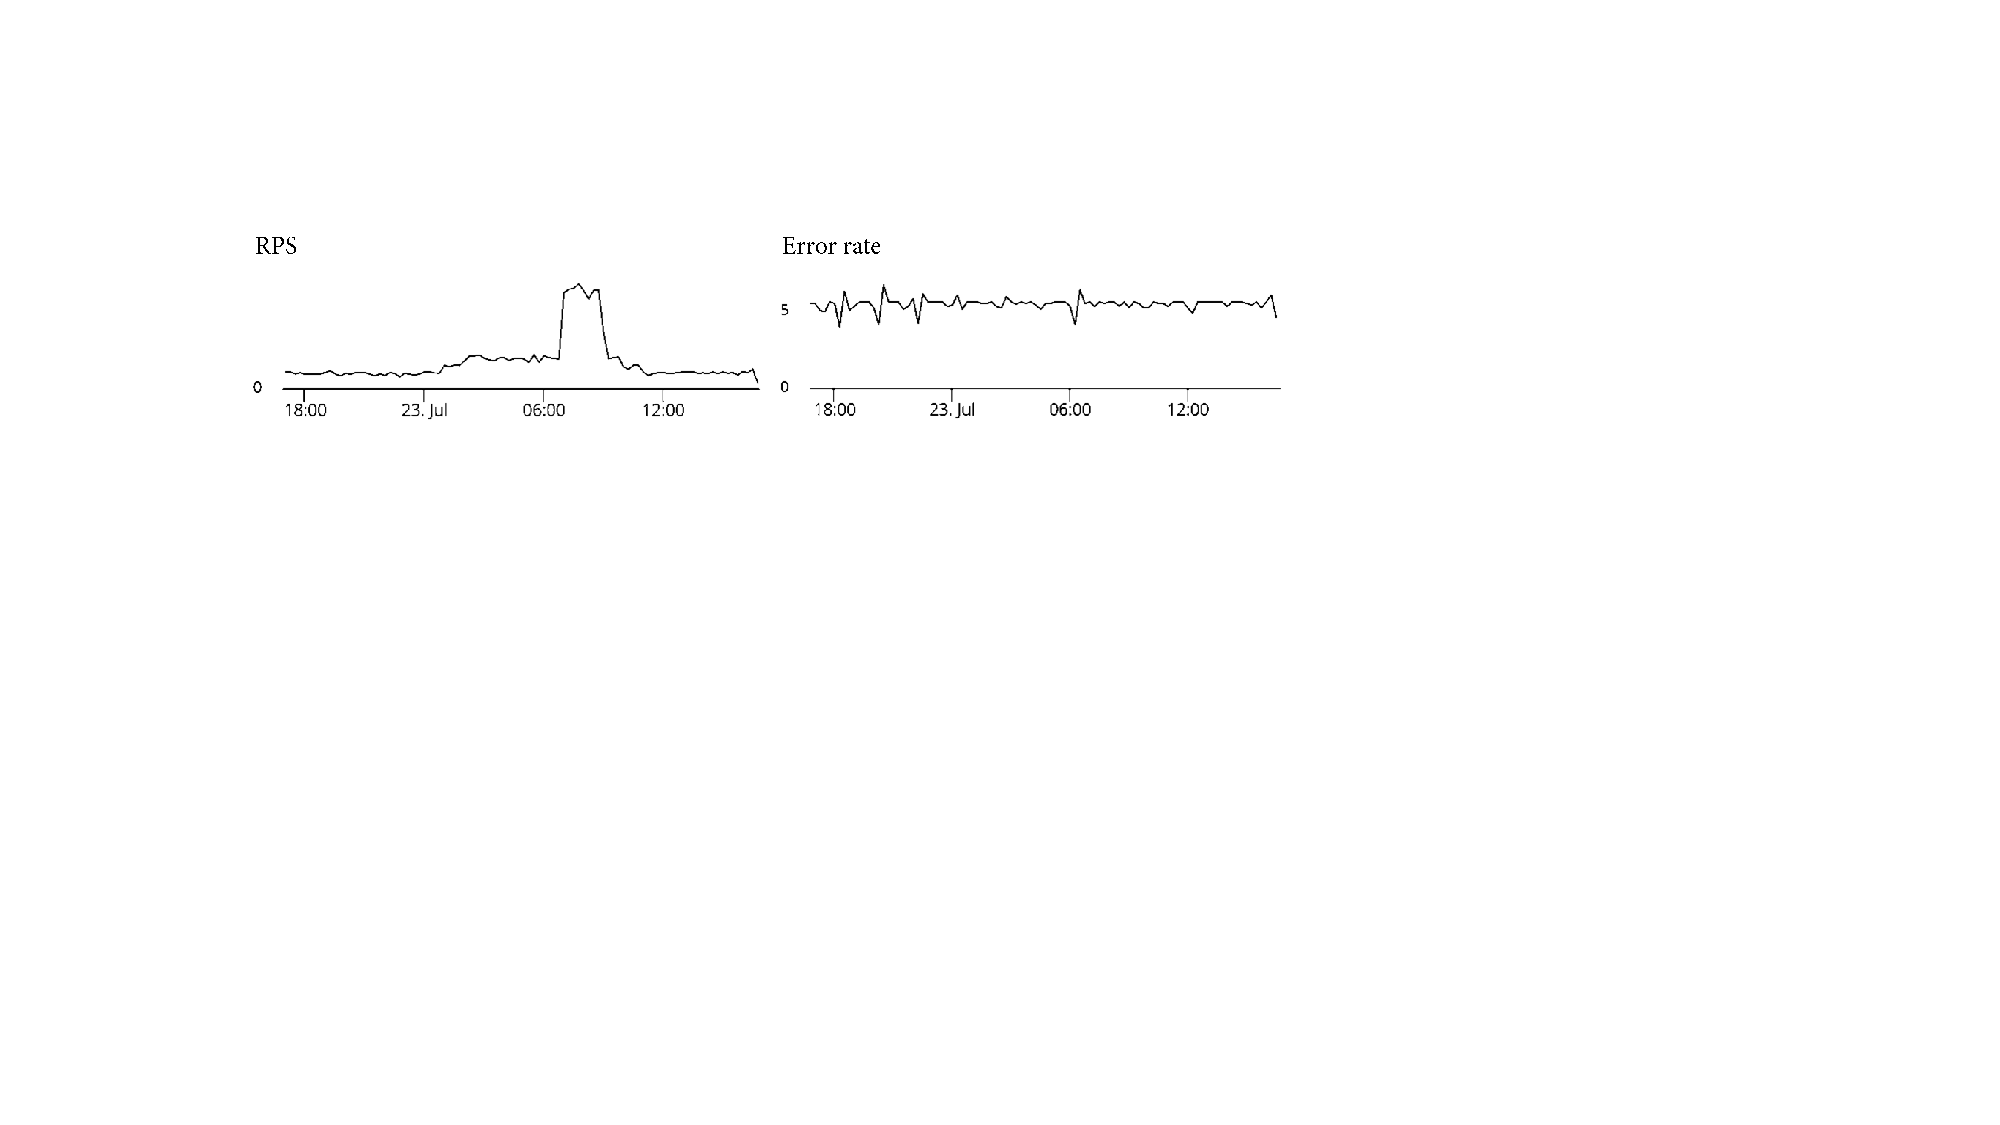
\includegraphics[width=1.0\textwidth]{gfx/chap2/rpsanderror.pdf}}
\caption{Examples of metric time series data. Response time (left) and error rate (right)~\cite{appoptics}.}
\label{fig:rpsanderror}
\end{figure}

We define a single observation of a metric as a value, timestamp, and sometimes list of properties that describe the observation, such as a source or tags. A time series is a set of observations $x_i$, each being recorded at specified time $t$~\cite{brockwell1991time}. We show examples of two time series from metric data in Figure~\ref{fig:rpsanderror}, requests per second and error rate. As metrics are simply numbers measured over intervals of time, they can be compressed, stored, processed, and retrieved efficiently. Metrics are optimized for storage and enable a longer retention of data, which can be used to build dashboards to reflect historical trends. The cost of metrics does not increase with the user traffic or any other system activity. Metrics, once collected, are more suitable for mathematical and statistical transformations such as sampling, aggregation, summarization, and correlation, which makes them better suited for monitoring and profiling purposes. Metrics are also suited to trigger alerts, as running queries against an in-memory time-series database is considerably more efficient than running a query against a distributed system storage, and then aggregating the results before deciding if an alert needs to be triggered~\cite{sridharan2018distributed,donut}.

Metrics can be sufficient for understanding the health of individual system components and application services. However, they are not sufficient to understand the lifetime of a request that traverses multiple systems, nor the semantics of the anomaly. Complex anomalies that propagate through several services and system components are more challenging to detect using solely metric data owing to the diminishing effect ~\cite{sridharan2018distributed,observability2020practical}.

\subsection{Logs} \label{ch:background:sec:observability:subsec:logs}
Logs are important in understanding and improving software systems. System operators and developers leverage the rich information in logs to generate workload information for capacity planning in large-scale systems~\cite{hassan2008industrial,nagappan2009efficiently}, monitor the overall system health~\cite{jiang2013automated}, perform anomaly detection~\cite{meng2019loganomaly,nedelkoski2019anomaly,nedelkoski2020loganomaly,nedelkoski2020selfsupervised,du2017deeplog,zhang2019robust,du2016spell,zhu2019tools}, analyze the root cause of a problem~\cite{Yuan2019AnAT,zhou2019latent,chen2019empirical}, reproduce failures~\cite{zhang2017pensieve}, improve the performance, reduce the energy consumption, address security issues~\cite{zhao2016non}, reconstruct workflows~\cite{bao2019miningworkflows}, and discover bugs~\cite{mohan2018finding}.

Logs are not only beneficial for developers and operators for successfully managing the system, but are also often needed to comply with legal regulations. For example, the Sarbanes-Oxley Act of 2002 specifies that the execution of telecommunication and financial applications must be logged to help protect the general public from errors and fraudulent practices~\cite{act2002sarbanes}.

In modern distributed systems, logs provide vital insights by capturing the state of the system for each service/component~\cite{zhu2019tools}. Logs are generally instrumented as per their usability by developers. Depending on the storage rules, they are processed, aggregated, and ultimately stored in a centralized data store from where they can be analyzed. Logs can originate from the application logic code, middleware, network communications (e.g., from switches), database communication, message brokers, caches, interaction with load balancers, and communication with security and authentication modules\cite{observability2020practical}. 

% \begin{figure}[!t]
% \centerline{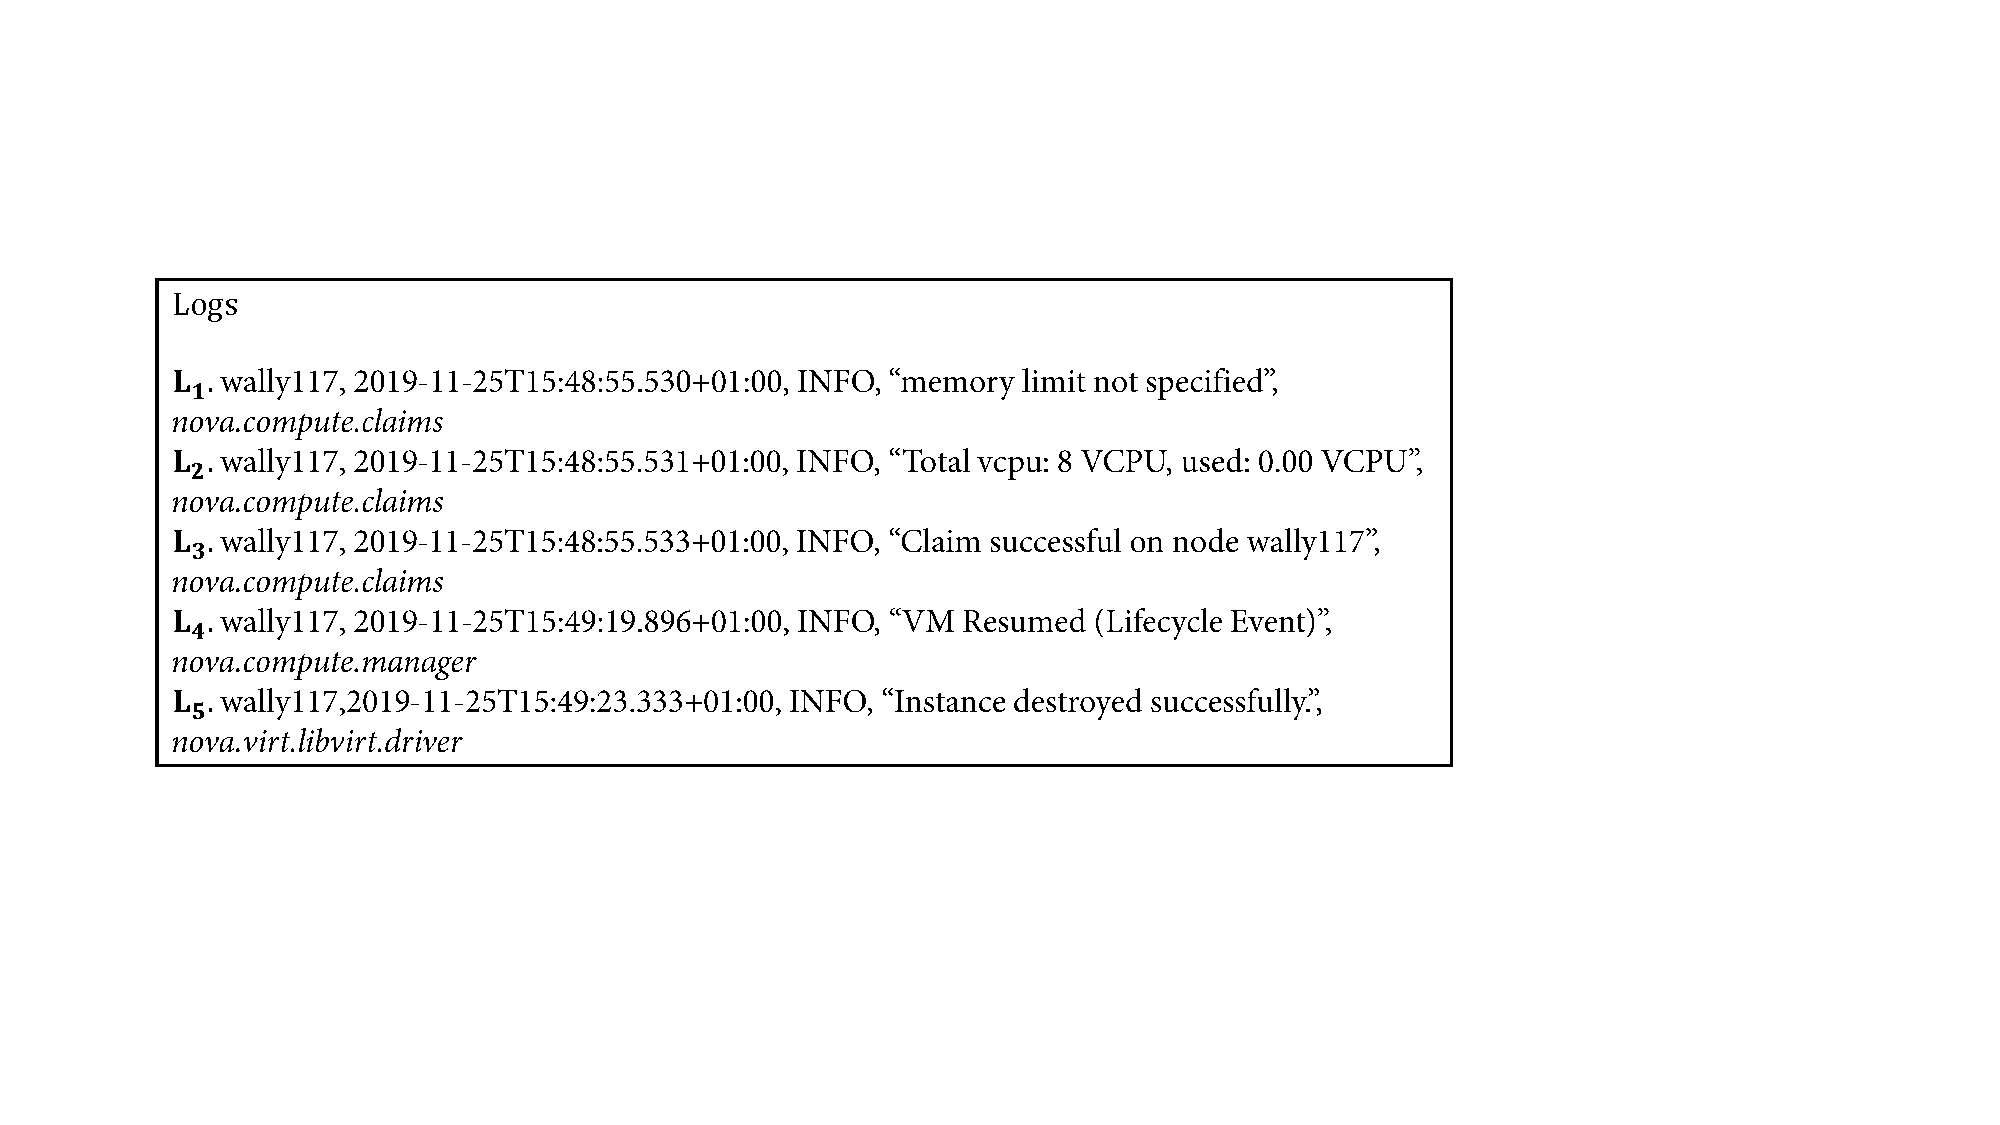
\includegraphics[width=1.0\textwidth]{gfx/chap2/log_lines.pdf}}
% \caption{Raw log messages}
% \label{fig:log_lines}
% \end{figure}

% \begin{table}[!t]
% \centering
% \caption{Raw log messages from OpenStack.}
% \resizebox{\columnwidth}{!}{%
% \begin{tabular}{l|l}
% \hline
% Nr. & \multicolumn{1}{c}{Log messages}                                                                      \\ \hline
% 1   & wally117, 2019-11-25T15:48:55.530, INFO, "memory limit not specified", nova.compute.claims            \\
% 2   & wally117, 2019-11-25T15:48:55.531, INFO, "Total vcpu: 8 VCPU, used: 0.00 VCPU", nova.compute.claims   \\
% 3   & wally117, 2019-11-25T15:48:55.533, INFO, "Claim successful on node wally117", nova.compute.claims     \\
% 4   & wally117, 2019-11-25T15:49:19.895, INFO, "VM Resumed (Lifecycle Event)", nova.compute.manager         \\
% 5   & wally117, 2019-11-25T15:49:23.333, INFO, "Instance destroyed successfully.", nova.virt.libvirt.driver \\ \hline
% \end{tabular}
% }\label{tab:log_lines}
% \end{table}

\begin{table}[!t]
\centering
\caption{Raw log messages from OpenStack cloud platform.}
\resizebox{\columnwidth}{!}{%
\begin{tabular}{cl}
\hline
Nr. & \multicolumn{1}{c}{Log messages}                                                                      \\ \hline
1   & 2019-11-25T15:48:55.530, INFO, "memory limit not specified", nova.compute.claims            \\
2   & 2019-11-25T15:48:55.531, INFO, "Total vcpu: 8 VCPU, used: 0.00 VCPU", nova.compute.claims   \\
3   & 2019-11-25T15:48:55.533, INFO, "Claim successful on node wally117", nova.compute.claims     \\
4   & 2019-11-25T15:49:19.895, INFO, "VM Resumed (Lifecycle Event)", nova.compute.manager         \\
5   & 2019-11-25T15:49:23.333, INFO, "Instance destroyed successfully.", nova.virt.libvirt.driver \\ \hline
\end{tabular}
}\label{tab:log_lines}
\end{table}

Independent on their origin type, logs contain free-form text with a timestamp, alongside other system-dependent fields. We show few typical log messages from a cloud computing infrastructure software (OpenStack~\cite{openstack}) in Table~\ref{tab:log_lines}. The first field is the timestamp when the log was generated, followed by a log level (INFO, WARNING, ERROR, etc.), payload or actual print statement written by developers, and name of the service from which was generated. Logs can also contain host names and IP addresses, class names, and other features.

Log is a string, blob of JSON, or typed key-value pairs, which enables to easily represent any data in the form of a log line. Most languages, application frameworks, and libraries are accompanied by support for logging~\cite{liu2019logzip}. Logs are also simple to instrument, as adding a log line is as trivial as adding a print statement. Logs exhibit high performances in terms of surfacing a highly granular information with a rich local context, provided that the search space is localized to events that occurred in a single service~\cite{sridharan2018distributed,hamooni2016logmine}.

However, logs, similar to the metric data, are system/service-scoped, which hinders the understanding of the full life cycle of a request that propagates through multiple connected services in the distributed system~\cite{sridharan2018distributed}. 
Often, various possible triggers across a highly interconnected graph of components are involved~\cite{gunawi2014bugs,sillito2020failures}. By solely observing discrete events that occurred in any given component at some point in time, it becomes challenging to determine all such triggers. This is the strongest drawback of log data.


\subsection{Distributed traces} \label{ch:background:sec:observability:subsec:traces}

\begin{figure}[!t]
\centerline{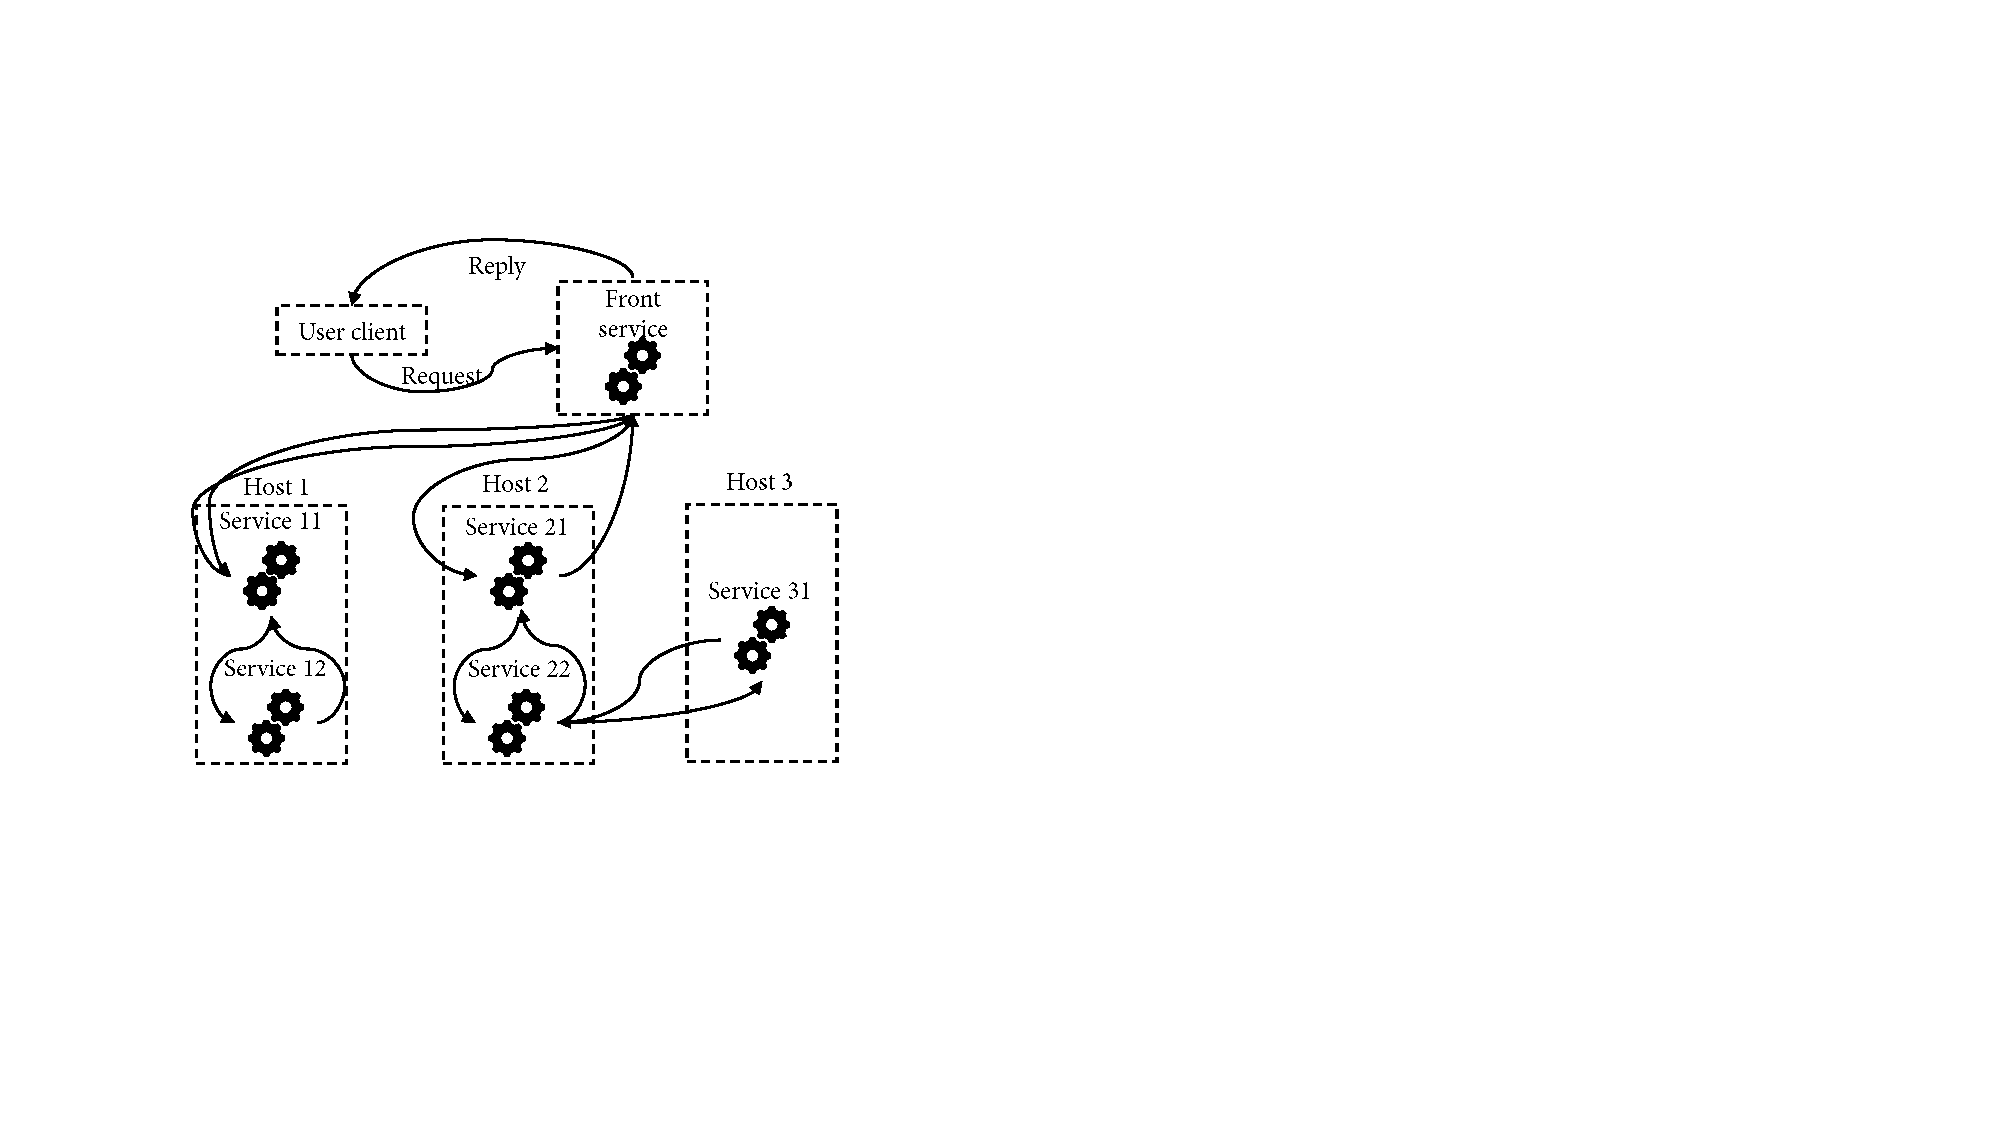
\includegraphics[width=0.8\textwidth]{gfx/chap2/pathmicroservice.pdf}}
\caption{Path through simple microservice system on behalf of the user request.}
\label{fig:pathmicroservice}
\end{figure}

The introduction of distributed traces helps address the drawbacks of the log data. They are a series of causally related distributed events that encode the end-to-end request flow through a distributed system. A single trace can provide visibility into the service response time to a request, path traversed by a request, and structure of a request~\cite{sigelman2010dapper,RepTrace}. The path of a request enables software developers and operators to understand the different services involved in executing a particular request. The structure of a request helps understand the junctures and effects of asynchrony in the execution of a request. The response time contained in the traces is related to the actual user experience, QoS, and can be considered as metric data~\cite{nedelkoski2019anomaly,nedelkoski2019anomalymultimodal}. 


A tracing infrastructure (e.g., Dapper~\cite{sigelman2010dapper}) for distributed services records information about all work in a system on behalf of a given initiator. In Figure~\ref{fig:pathmicroservice}, we show an example of a system with four servers and six microservices. We describe the path of invocation of services and simple trace. A user sends a request at the frontend. The front service sends two calls to microservices in hosts 1 and 2. Service 11 on host 1 calls service 12 (e.g., database) and responds to the request from the frontend. However, services 21 and 22 require work from service 31 at host 3, before a reply is sent to the frontend. A simple trace for this request will be a collection of message identifiers and timestamped events for every message sent and received at each service.


\begin{figure}[!t]
\centerline{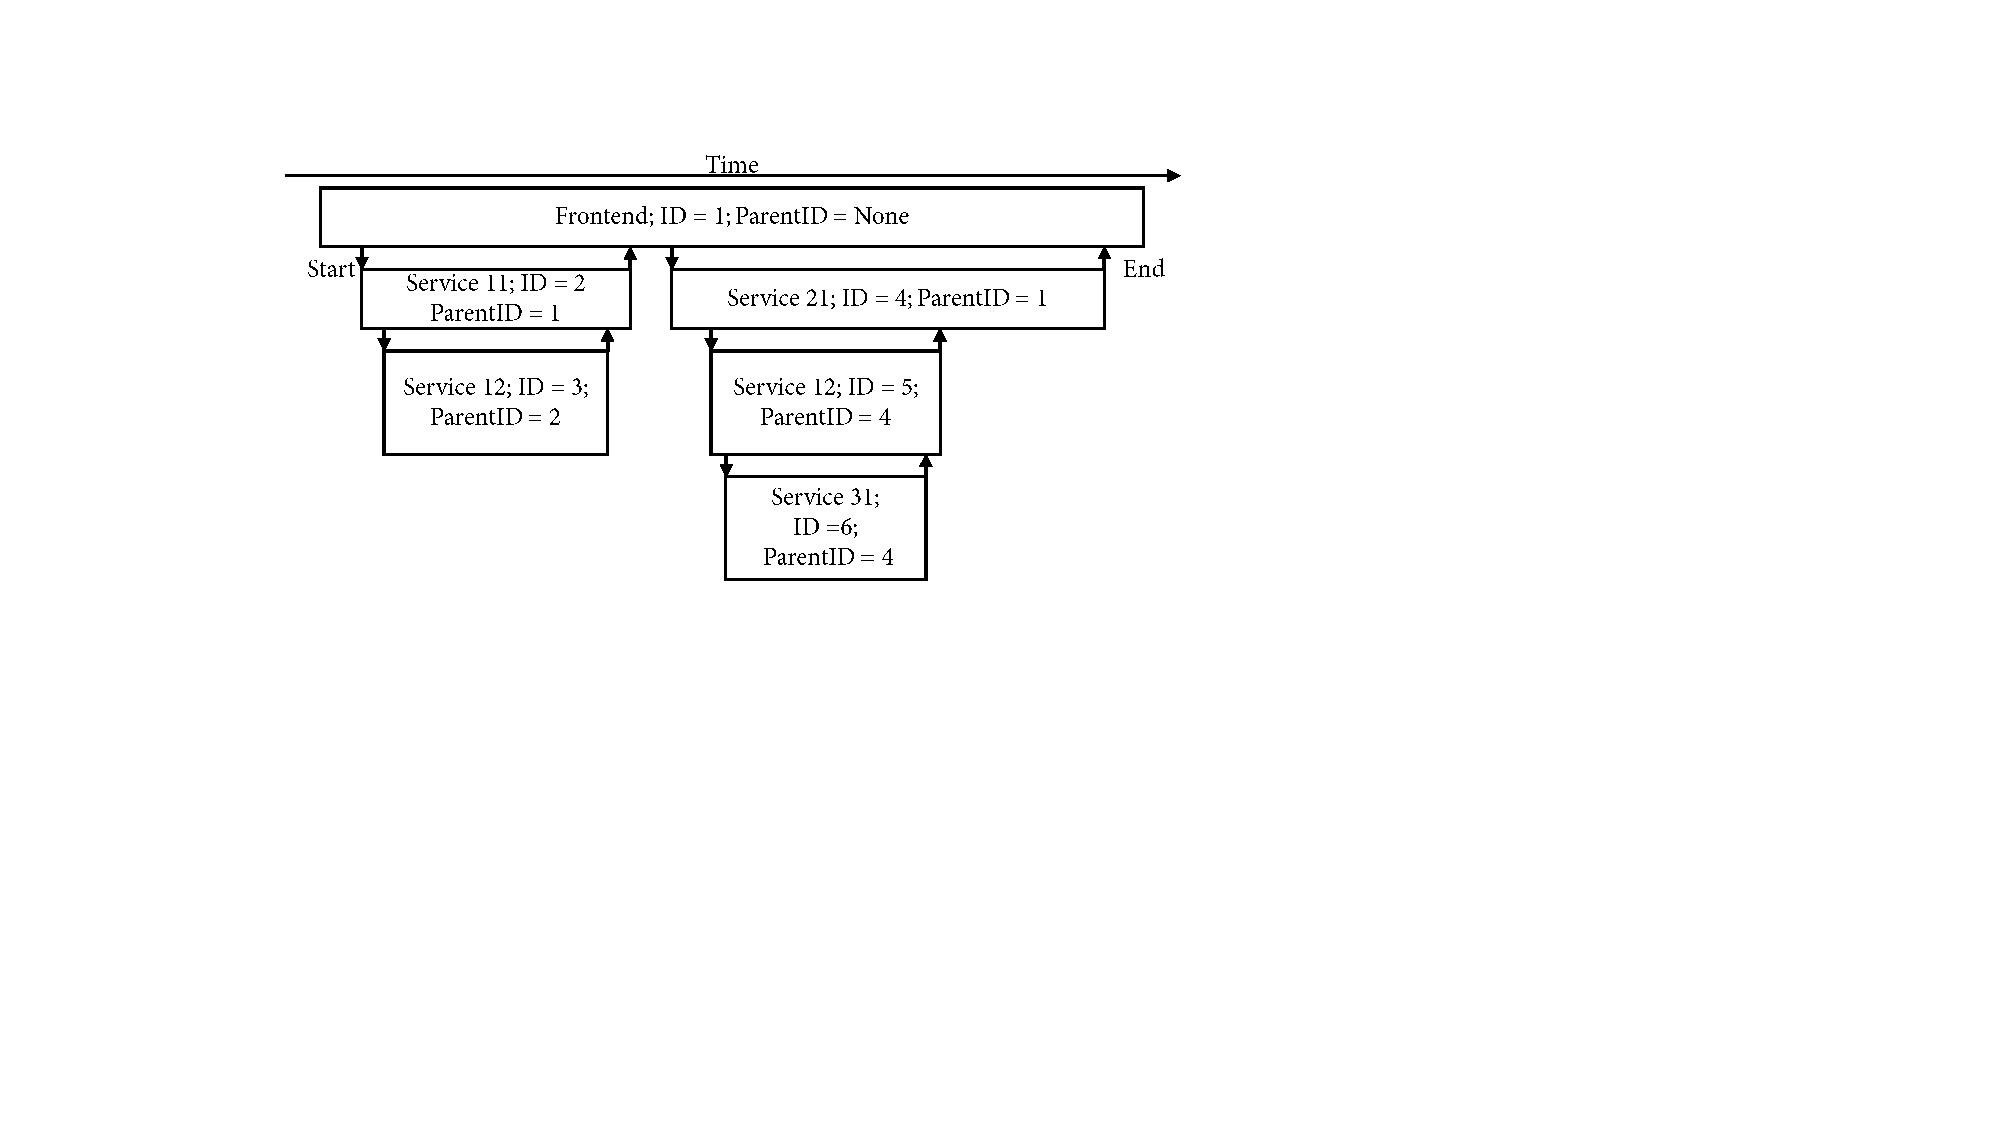
\includegraphics[width=1.0\textwidth]{gfx/chap2/tracetree.pdf}}
\caption{Causal and temporal relationships between events in a trace.}
\label{fig:temporalevents}
\end{figure}

\begin{figure}[!b]
\centerline{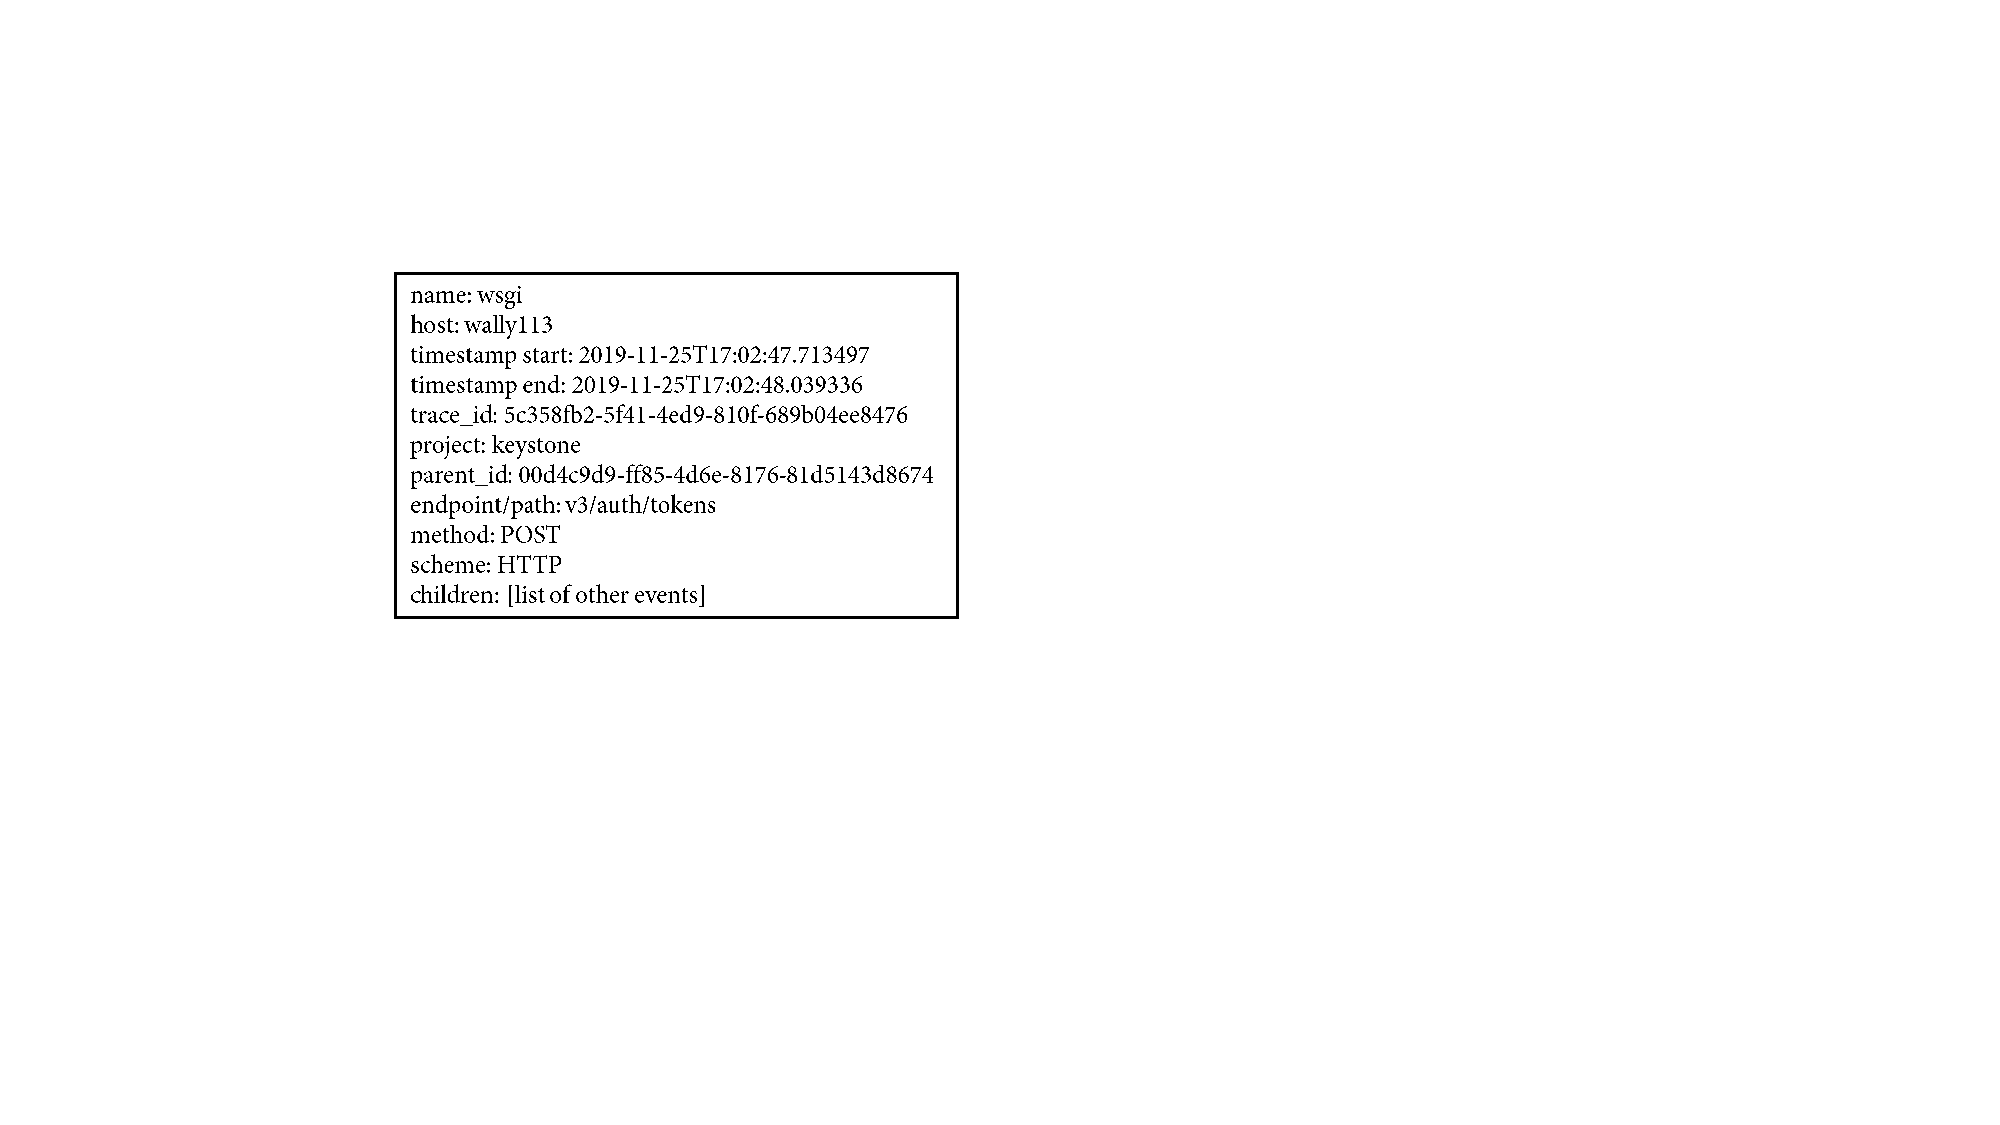
\includegraphics[width=0.6\textwidth]{gfx/chap2/single_event.pdf}}
\caption{Detailed view of a single event from a trace.}
\label{fig:singleevent}
\end{figure}


Such execution path with distributed tracing can be naturally described as a graph. In a trace graph, the nodes are basic units of work, referred to as events or spans. Each service invocation produces one span in the trace. The edges indicate a causal relationship between services. We illustrate spans forming the structure of a larger trace in Figure~\ref{fig:temporalevents}. Tracing records a human-readable span name for each span, as well as a Span ID and Parent ID. To reconstruct the causal relationships between the individual spans in a single distributed trace, we need to follow the parent--child relationship between the spans (representing a service invocation). Spans created without a Parent ID are known as root spans. All spans associated with a specific trace also share a common identifier Trace ID. All these IDs are probabilistically unique 64-bit integers~\cite{sigelman2010dapper}.

Figure~\ref{fig:singleevent} provides a more detailed view of the logged events in a typical trace span. Each span within the trace is described by its start and stop times, name of the host of the service, name of the service/project, HTTP endpoint, and list of its children spans/services. If application owners choose to augment the trace with their annotations, these are also recorded with the rest of the span data. 

\begin{figure}[!htbp]
\centerline{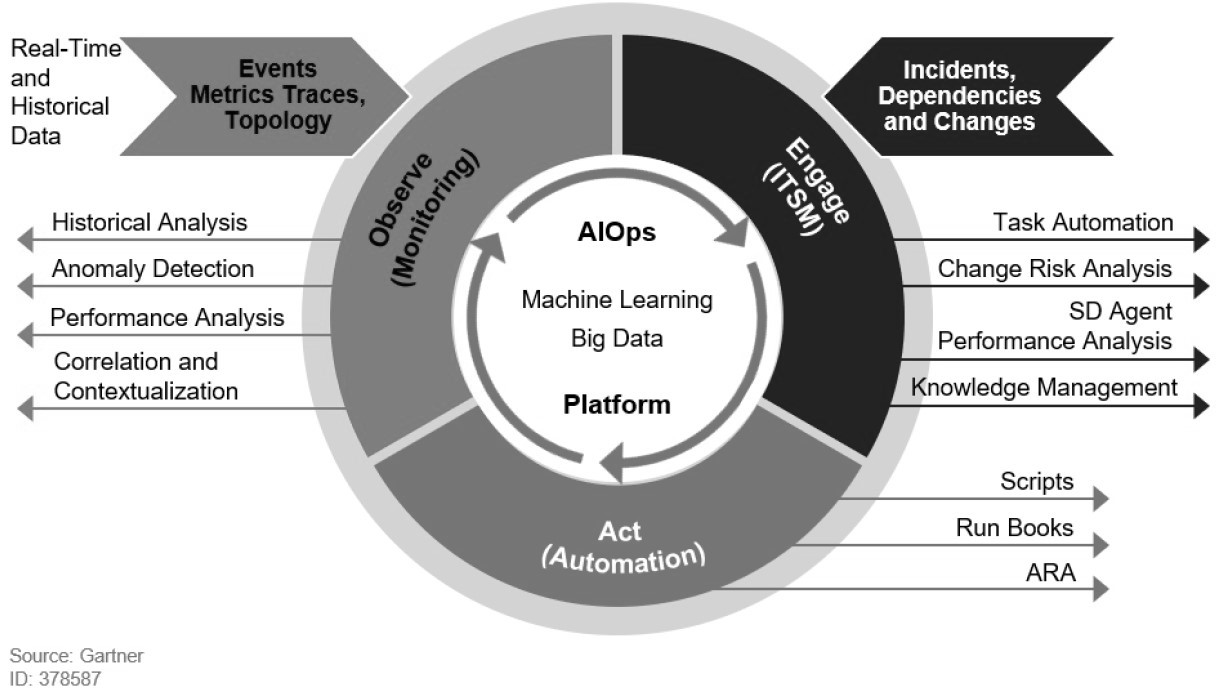
\includegraphics[width=1.0\textwidth]{gfx/chap2/aiopsgartner.jpg}}
\caption{Overview of AIOps tasks~\cite{gartnerinc,gartnermarketguide}.}
\label{fig:overviewaiops}
\end{figure}

\section{Artificial intelligence for IT systems}\label{ch:background:sec:aiops}
The amount and descriptive power of the observability data sources are favourable for the use of artificial intelligence methods. In this context, the term AIOps was coined by Gartner~\cite{gartnermarketguide} to address the DevOps challenges with AI. AIOps aims to achieve high service intelligence, customer satisfaction, and engineering productivity. However, numerous challenges still need to be overcome.





The software industry is still at the early stage of innovating and adopting AIOps solutions. According to FutureScape and Gartner predictions~\cite{futurescape2018worldwide, gartnerinc}, by 2024, 60\% of the companies will adopt ML/AI analytics for their development, maintenance, and operation tasks.

\subsection{AIOps tasks}\label{ch:background:sec:aiops:subsec:tasks}
AIOps can enhance a broad range of IT operation processes and tasks, including performance analysis, anomaly detection, event correlation and analysis, IT service management, and automation (see Figure~\ref{fig:overviewaiops}). The focus of AIOps, according to Gartner~\cite{gartnerinc,gartnermarketguide}, includes:
\begin{itemize}
    \item Basic and advanced statistical analyses: a combination of univariate and multi-variate analyses including correlations and computing other statistic indicators.
    \item Anomaly detection: use of the observed normal system behavior to initially develop a model, and then flag departures from the normal system behavior~\cite{yeanomalycloud,liu2016anomaly,vrushali2016anomaly,zhou2017anomaly}.
    \item Root cause localization: isolation of links of dependency that represent genuine causal relationships in terms of providing recipes for an effective intervention when an anomaly is detected~\cite{lou2010mining,fraenkel2004root,dalal2013empirical,nedelkoski2020rca,meng2020localizing}.
    \item Prescriptive advice and healing: classification of anomalies and root causes into known categories, relating them with solutions, analyzing the possible solutions for applicability, and offering them in a prioritized form for usage of remediation~\cite{sidiroglou2009assure,dashofy2002towards}.
    \item Topology: for the patterns detected to be relevant and actionable, a context must be placed around them. The context is topology. Without the context, the detected patterns, although valid, may be unhelpful and even distracting. Deriving patterns from data within a topology will reduce the number of patterns, establish relevancy, and illustrate hidden dependencies. Using topology as a part of the causality determination can largely increase its accuracy and effectiveness. Capturing where events occurred and their up- and downstream dependencies using graph and bottleneck analyses can provide valuable insights to focus the remediation efforts~\cite{donnet2005efficient,donnet2005improved,donnet2007internet, keller2007methods,muntonimining}.
\end{itemize}

\newpage

\section{Anomaly detection}\label{ch:background:sec:anomalydetection}
Anomaly detection has been a lasting yet active research field in various research domains for several decades. As an application-driven research field, numerous methods have been proposed including those in statistics, computer systems, healthcare, banking, and earth sciences~\cite{Aggarwal:2013:OA:2436823}. Anomaly detection is used as a general method for various techniques and approaches that share the aim of finding unusual observations in given data. A general widely accepted definition of anomaly has been reported by Hawkings~\cite{hawkins1980identification}:

\begin{center}
\textit{
"An outlier (anomaly) is an observation which deviates so much from
other observations as to arouse suspicions that it was generated by a
different mechanism."}
\end{center}


Predecessor definitions have also been reported (e.g., that by Grubbs in 1969~\cite{grubbs1969procedures}):

\begin{center}\textit{ 
"An outlying observation, or "outlier" (anomaly), is one that appears to deviate markedly from other members of the sample in which it occurs."}   
\end{center}

These definitions suggest that anomaly detection is a quite old method in computer science and statistics. However, recently, the importance of anomaly detection significantly increased with the appearance of the internet, online services, big data, large computer systems, and their economical impact. Numerous online services rely on combinations of anomaly detection methods. For example, cloud platforms utilize anomaly detection to improve their resilience and reliability, fraud detection is extensively used in the banking sector, and intrusion detection tools are implemented to prevent cyber attacks. Depending on the application and context of use, the term "anomaly" is often substituted by outlier, exception, noise, abnormality, and deviation. 

A common anomaly detection approach is to define a region representing the normal behavior and declare any observation in the data that does not belong to the normal region as an anomaly. However, several properties make this apparently simple approach challenging to use~\cite{chandola2009anomaly,pang2020deep}:
\begin{itemize}
    \item Defining a model that captures every possible normal behavior is challenging as it is not possible to identify every possible normal behaviour in most applications.
    \item When anomalies are results of malicious actions, the malicious adversaries often adapt to make the anomalous observations appear as normal.
    \item In numerous domains, the normal behavior continuously evolves and a current notion of normal behavior might not be sufficiently representative in the future.
    \item The availability of labeled data for training/validation of models used by anomaly detection techniques is often a major issue.
    \item The data contain noise, which tends to be similar to the actual anomalies, and hence is challenging to distinguish and remove.
\end{itemize}

Considering the above challenges, the anomaly detection problem, in its most general form, is not simple. Therefore, most of the existing anomaly detection techniques solve a specific formulation of the problem, which is application-dependent. 

\begin{figure}[!t]
\centerline{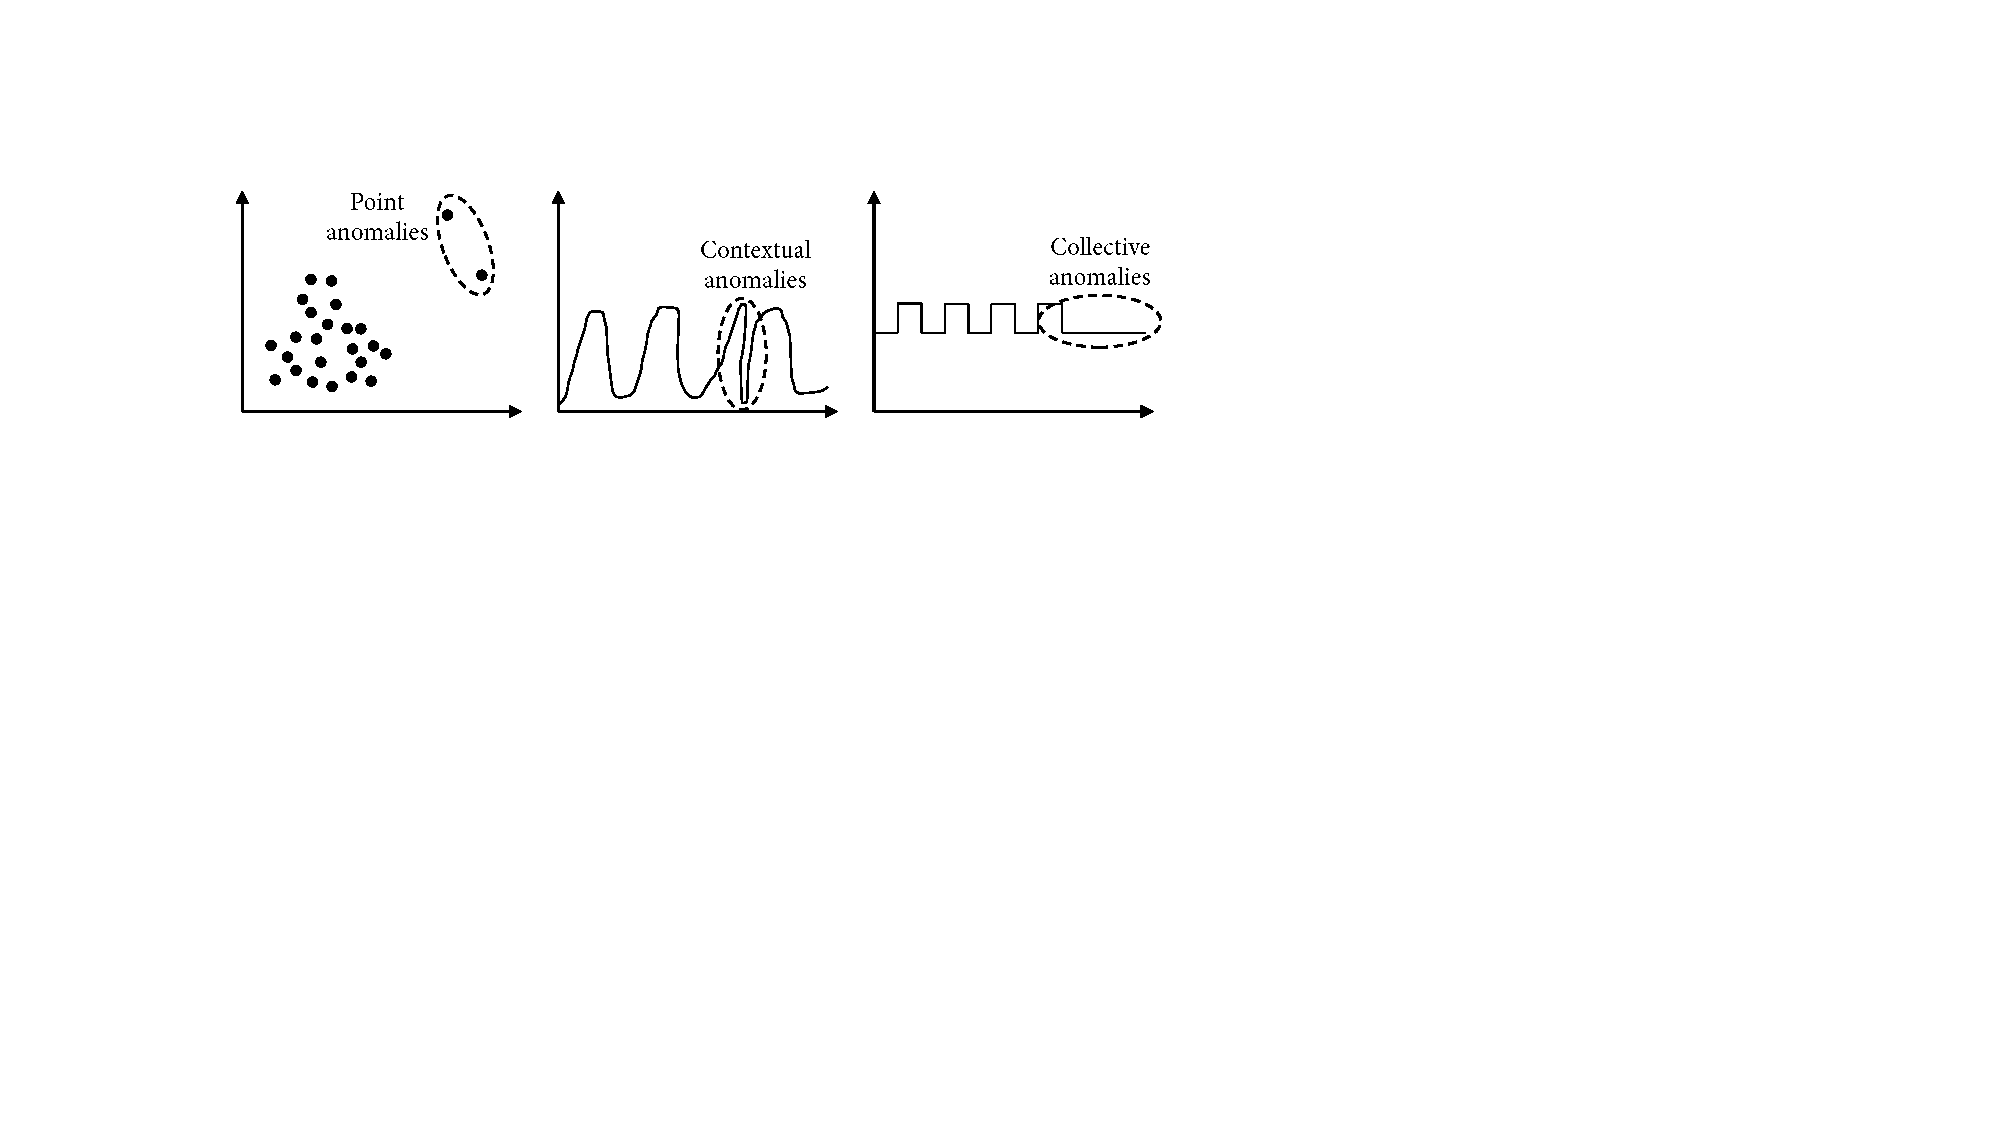
\includegraphics[width=1.0\textwidth]{gfx/chap2/typesofanomalies.pdf}}
\caption{Example of point anomalies (left). Example of a contextual anomaly (middle, the value of the data instance at the minimum is not anomalous; however, it is anomalous in the region outlined by the dashed line). Example of a collective anomaly (right); the absence of a whole group of data points forms an anomaly.}
\label{fig:typesofanomalies}
\end{figure}

Furthermore, anomalies appear in numerous different forms and contexts. In general, regarding the type of anomalies that could possibly arise, three different types are considered~\cite{chandola2009anomaly} (Figure~\ref{fig:typesofanomalies}):
\begin{itemize}
%Give examples in system data
    \item \textbf{Point anomalies} are data points that appear isolated from the bulk of the data.
    \item \textbf{Contextual anomalies}, sometimes referred to as conditional anomalies, are data points whose values are anomalous only in a specific contextual relation. Contextual features might be time, location, or broader data structure.
    \item \textbf{Collective anomalies} consist of a sequence of data points that only as a group, not as individual points, can be regarded anomalous.
\end{itemize}

Point anomalies have been extensively investigated as numerous methods assume that data points are independent instances~\cite{chandola2009anomaly,gornitz2019one}. However, data points can have strong dependencies. Therefore, it is expected to handle these data points in a collective or contextual manner. For example, asynchrony logs might not have emphasized contextual dependencies, while metric and trace data are inherently dependent.

The labels associated with a data instance denote whether that instance is normal or anomalous. Notably, the acquisition of labeled data that are accurate as well as representative of all types of behaviors is often prohibitively costly~\cite{chandola2009anomaly}. The labeling in all domains is often carried out manually by a human expert and hence a substantial effort is required to obtain the labeled training data set. Typically, the provision of a labeled set of anomalous data instances that cover all possible types of anomalous behavior is more challenging than the provision of labels for the normal behavior. Moreover, the anomalous behavior is often dynamic in nature; e.g., new types of anomalies may arise, for which no labeled training data exist. In certain cases (e.g., in air traffic safety), anomalous instances may translate to catastrophic events, and hence are rare~\cite{ruff2020unifying}. The provision of labeled data from distributed systems is costly and challenging owing to mostly practical limitations. As already mentioned, such systems undergo constant changes, e.g., software updates and hardware modernization, where labeled data become deprecated over time. Moreover, injection of anomalies to obtain data points is not possible as most running systems cannot risk possible downtimes~\cite{gunawi2014bugs,meng2019loganomaly,sillito2020failures}. Based on the extent to which the labels are available, anomaly detection techniques can operate in one of the following three modes: supervised, semi-supervised, and unsupervised anomaly detection, discussed below.

\subsection{Supervised anomaly detection} 
\label{ch:background:sec:anomalydetection:subsec:supervised}
The methods for supervised anomaly detection are similar to building predictive models~\cite{chandola2009anomaly}. These techniques assume the availability of a training data set, which has labeled instances for normal as well as anomaly classes. A typical approach in such cases is to develop a predictive model for binary classification, which aims to learn the distinctions between the normal and anomaly classes.
Any unseen data instance is compared against the model to determine which class it belongs to. 

Two major issues exist in supervised anomaly detection. First, issues emerge owing to imbalanced class distributions. Second, the provision of accurate and representative labels, particularly for the anomaly class, is usually challenging~\cite{theiler2003resampling, steinwart2005classification}. 

\subsection{Semi-supervised anomaly detection}
\label{ch:background:sec:anomalydetection:subsec:semisupervised}
In numerous real-world applications including anomaly detection in distributed systems, the operators have access to some verified (i.e., labeled) normal or anomalous samples in addition to the unlabeled data. The inclusion of these samples together with the bulk of unlabeled data leads to a semi-supervised anomaly detection problem. 

Considering $N$ (mostly normal but possibly containing some anomalous samples) unlabeled samples $x_1,\dots, x_N$ and $M$ labeled samples $(\hat{x_1}, \hat{y_1}),\dots,(\hat{x_M}, \hat{y_M})$, where $\hat{y} = 0$ and $\hat{y} = 1$ denote normal and anomalous samples, respectively, the task is to learn a model that compactly characterizes the normal class. The typical approach used in semi-supervised techniques is to develop a model for the class corresponding to the normal behavior and use the model to identify anomalies in the test data. The term semi-supervised anomaly detection has been used to describe two different anomaly detection settings. Most existing semi-supervised AD methods are instances of learning from positive (i.e., normal) and unlabeled examples. A few studies have been carried out on the general semi-supervised AD setting where labeled anomalies are also utilized. However, existing deep approaches are domain- or data-type-specific~\cite{ruff2019deep,chandola2009anomaly}. A limited set of anomaly detection techniques assume availability of only the anomaly instances for training due to the challenges to obtain anomalies that cover all cases~\cite{ruff2019deep}.

\subsection{Unsupervised anomaly detection}
\label{ch:background:sec:anomalydetection:subsec:unsupervised}
Techniques that operate in the unsupervised mode do not require labeled training data, and thus are most widely applicable~\cite{ruff2020unifying,ruff2019deep,ruff-etal-2019-self,nedelkoski2019anomaly,nedelkoski2019anomalymultimodal,nedelkoski2020loganomaly,meng2019loganomaly}. The techniques in this category use the implicit assumption that normal instances are far more frequent than anomalies in the test data~\cite{ruff2020unifying}. If this assumption is not true, such techniques suffer from a high false alarm rate. Numerous semi-supervised techniques can be adapted to operate in an unsupervised mode using a sample of the unlabeled data set as training data. Such adaptation assumes that the test data contains few anomalies. The model learnt during the training is robust to these few anomalies. However, a large gap exists between the supervised and unsupervised anomaly detection methods. The supervised anomaly detection is largely favored  under the assumption that all data are labeled~\cite{ruff2020unifying}.

\subsection{Deep anomaly detection}
\label{ch:background:sec:anomalydetection:subsec:deepanomaly}
The performances of traditional algorithms in detecting outliers can still be improved on the sequence and image datasets as they cannot capture complex patterns in the data~\cite{pang2020deep}. Moreover, as the volume of data increases, for example, to gigabytes, it becomes almost impossible for the traditional methods to scale to such large-scale data to find anomalies~\cite{chalapathy2019deep}.
To mitigate these issues, deep learning for anomaly detection, shortly \emph{deep anomaly detection}, aims to learn feature representations or anomaly scores through neural networks. A large number of deep anomaly detection methods have been introduced, with significantly higher performances than those of the conventional anomaly detection methods~\cite{pang2020deep}. However, the lack of a well-defined representative normal boundary poses challenges for both conventional and deep learning-based algorithms.

Deep neural networks leverage complex compositions of linear/nonlinear functions that can be represented by a computational graph to learn expressive representations~\cite{Goodfellow-et-al-2016}. The basic building blocks of deep learning are activation functions and layers. Activation functions determine the output of computational graph nodes (i.e., neurons in neural networks) for given inputs. They can be linear or nonlinear functions. Popular activation functions include linear, sigmoid, tanh, rectified linear unit (ReLU), and its variants. A layer in neural networks refers to a set of neurons stacked in some forms. Commonly used layers include fully connected, convolutional \& pooling, and recurrent layers. These layers can be leveraged to build different popular neural networks. For example, multi-layer perceptron (MLP) networks are composed of fully connected layers, convolutional neural networks (CNNs) have varying groups of convolutional \& pooling layers, and recurrent neural networks (RNNs), e.g., vanilla RNN, gated recurrent units (GRUs), and long-short-term memory (LSTM), are based on recurrent layers. We refer the reader to Goodfellow et al.~\cite{Goodfellow-et-al-2016} for a detailed description of the neural networks.

For a dataset $\mathcal{X} =\{\mathbf{x_1}, \mathbf{x_2}, \cdots, \mathbf{x_N}\}$ with $\mathbf{x_i} \in \mathbb{R}^{D}$ and $\mathcal{Z} \in \mathbb{R}^{K}$ as a representation space, deep anomaly detection aims to learn a feature representation mapping function $\phi(\cdot): \mathcal{X} \mapsto \mathcal{Z}$ or anomaly score learning function $\tau(\cdot):\mathcal{X} \mapsto \mathbb{R}$ in a manner that anomalies can be easily differentiated from the normal data instances in the $\phi$ or $\tau$ space, where $\phi$ and $\tau$ are a neural-network-enabled mapping function with $H \in \mathbb{N}$ hidden layers and their weight matrices $\Theta=\{\mathbf{M}^{1}, \mathbf{M}^{2}, \cdots, \mathbf{M}^{H}\}$, respectively. In the case of learning the feature mapping $\phi(\cdot)$, an additional step is required to calculate the anomaly score of each data instance in the new representation space, while $\tau(\cdot)$ can directly infer the anomaly scores with raw data inputs. 

Pang et al.~\cite{pang2020deep} provided an exhaustive overview of deep anomaly detection methods grouped by three conceptual paradigms: deep learning for feature extraction, learning feature representations of normality, and end-to-end anomaly score learning. We discuss below the main concepts and methods for each group. For details, we refer the reader to more comprehensive reviews of the literature~\cite{pang2020deep,chalapathy2019deep,ruff2020unifying}.

\subsubsection{Deep learning for feature extraction}
\label{ch:background:sec:anomalydetection:subsec:deepanomaly:subsubsecfeature}
This category of studies aims to leverage deep learning to extract low-dimensional feature representations from high-dimensional data for downstream anomaly detection. The feature extraction and anomaly scoring are fully disjointed and independent on each other. Thus, the deep learning components are used only for dimensionality reduction. Formally, the approach can be represented by

\begin{equation}\label{eqn:featureextraction}
\centering
\mathbf{z} = \phi(\mathbf{x}; \Theta),
\end{equation}

where $\phi:\mathcal{X} \mapsto \mathcal{Z}$ is a deep-neural-network-based feature mapping function, with $\mathcal{X}\in \mathbb{R}^{D}$, $\mathcal{Z} \in \mathbb{R}^{K}$, and normally $D \gg K$. An anomaly scoring method $f$ that has no connection to the feature mapping $\phi$ is then applied onto the new space to calculate anomaly scores.

Compared to the dimension reduction methods, popular for anomaly detection, such as principal component analysis (PCA)~\cite{jolliffe2016principal}, deep learning techniques have exhibited substantially better capabilities in extracting semantic-rich features and nonlinear feature relations~\cite{bengio2013representation,Goodfellow-et-al-2016}.

\subsubsection{Learning feature representations of normality}\label{ch:background:sec:anomalydetection:subsec:deepanomaly:featuresrepresentations}
The deep anomaly detection methods in this category couple feature learning with anomaly scoring to some extent, which are different from the methods in the last section, which fully decouple these two modules. 

This category of methods learn the representations of data instances by optimizing a generic feature learning objective function that is not primarily designed for anomaly detection, but the learned representations can be still utilized for the anomaly detection as they are forced to capture some key underlying data regularities. Formally, this framework can be represented by

\begin{equation}
\{\Theta^*, \mathbf{W}^*\} = {\Theta,\ \mathbf{W}} \sum_{\xvec \in \mathcal{X}}\ell\Big(\psi\big(\phi(\mathbf{x};\Theta);\mathbf{W}\big)\Big),
s_{\mathbf{x}} = f(\mathbf{x}, \phi_{\Theta^*}, \psi_{\mathbf{W}^*}) \label{eqn:genericfeature2},
\end{equation}

where $\phi$ maps the original data onto the representation space $\mathcal{Z}$, $\psi$ parameterized by $\mathbf{W}$ is a surrogate learning task that operates on the $\mathcal{Z}$ space and is dedicated to enforce the learning of underlying data regularities, $\ell$ is a loss function relative to the underlying modeling approach, and $f$ is an anomaly scoring function that utilizes these two functions with the trained parameters $\Theta^*$ and $\mathbf{W}^*$ to calculate the anomaly score $s$. This approach includes methods driven by several perspectives, including data reconstruction, generative modeling, predictability modeling, and self-supervised classification.

\subsubsection{End-to-end anomaly score learning}
\label{ch:background:sec:anomalydetection:subsec:deepanomaly:subsubsec:anomalyscore}
This approach aims to learn scalar anomaly scores in an end-to-end manner. Compared to anomaly measure-dependent feature learning, the anomaly scoring in this type of approach is not dependent on existing anomaly measures. It has a neural network that directly learns the anomaly scores. Novel loss functions are often required to drive the anomaly scoring network. Formally, this category of methods aims to learn an end-to-end anomaly score learning network: $\tau(\cdot; \Theta):\mathcal{X} \mapsto \mathbb{R}$. The underlying framework can be represented as

\begin{gather}\label{eqn:scorelearning1}
    \Theta^* = \argmin_{\Theta} \sum_{\xvec \in \mathcal{X}} \ell\big( \tau(\mathbf{x};\Theta) \big),\\
    s_{\xvec} = \tau(\mathbf{x};\Theta^*)\label{eqn:scorelearning2}.
\end{gather}


\subsubsection{Autoencoders}\label{ch:background:sec:anomalydetection:subsec:deepanomaly:subsubsec:autoencoders}
Autoencoders are utilized as a neural architecture throughout this thesis. This type of approach aims to learn some low-dimensional feature representation space on which the given data instances can be well reconstructed. This is a widely used technique for data compression or dimension reduction~\cite{hinton2006reducing,wang2014generalized,sakurada2014anomaly}. The heuristic for using this technique in anomaly detection is that the learned feature representations are enforced to learn important regularities of the data to minimize reconstruction errors. It is challenging to reconstruct anomalies from the resulting representations, and thus they have large reconstruction errors.


\begin{figure}[!t]
\centerline{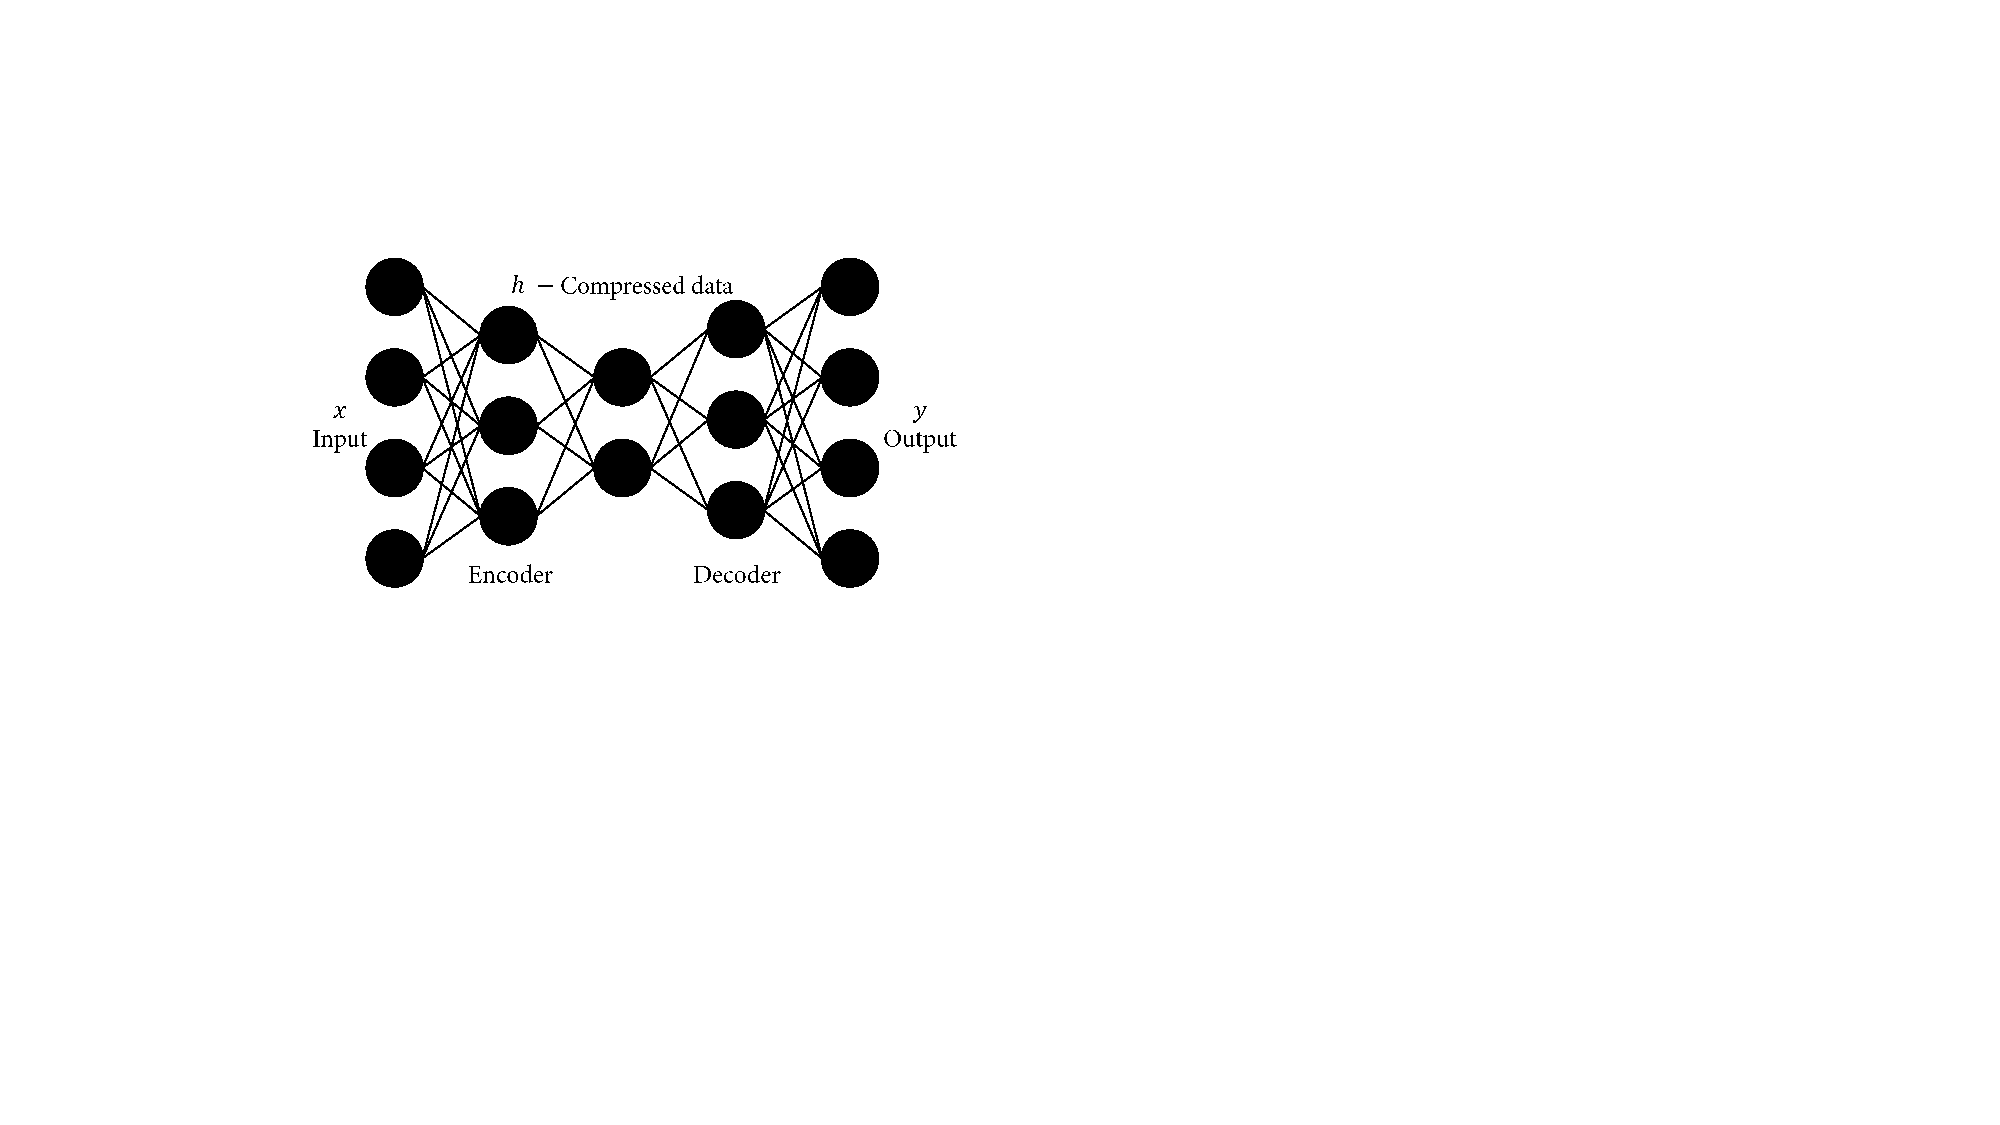
\includegraphics[scale=1.1]{gfx/chap2/autoencoder.pdf}}
\caption{Architecture of an under-complete autoencoder.}
\label{fig:autoencoder}
\end{figure}

It is assumed that normal data instances can be better restructured from the compressed feature space than anomalies. In autoencoders, the output (target) value is set equal to the input, i.e., $y_i=x_i$~\cite{hinton2006reducing} (see Figure~\ref{fig:autoencoder}). 
The autoencoder learns a function $h(w,b(x)) \simeq x$. 
In other words, it aims to learn an approximation to the identity function, to output $y$ similar to $x$.
The identity function seems a trivial function to learn. However, by placing some constraints, e.g., by limiting the number of hidden units or introducing regularization, we can extract some valuable features from the data.
Modern autoencoders have generalized the idea of encoder and decoder beyond deterministic functions to stochastic mapping.
One approach to obtain useful features, as mentioned, is to have a smaller h-dimension than x. 
This is referred to as under-complete autoencoder. Learning the under-complete representation forces the autoencoder to capture the most important features of the data. 
The learning consists simply of minimizing the error function by back-propagation.

If the hidden layer has a higher dimensionality than that of the input, the under-complete autoencoder will not learn salient features because it will only trivially copy the input to the output. A possible solution to train autoencoders is to include regularization. Rather than limiting the model capacity, regularized autoencoders use a loss function that encourages the model to have other properties besides the ability to copy its input to its output. These properties include sparsity of the representation, robustness to noise, and handling missing inputs. 
Autoencoders have been successfully applied to dimensionality reduction, anomaly detection, and information retrieval. For example, a lower-dimension representation can improve the performances of numerous tasks, such as classification, so that the models will consume less memory and run-time~\cite{ruff2020unifying,pang2020deep}.

\newpage

\subsubsection{Self-supervised learning}
\label{ch:background:sec:anomalydetection:subsec:deepanomaly:subsubsec:selfsupervised}
Self-supervised learning is learning of representations by solving auxiliary tasks. These auxiliary prediction tasks do not require ground-truth labels for learning and thus can be applied to unlabeled data, which makes the self-supervised learning suitable for anomaly detection.
Self-supervised methods introduced for visual anomaly detection train multi-class classification models based on pseudo-labels that correspond to various geometric transformations (e.g., flips, translations, and rotations)~\cite{hendrycks2019using}.
In a broader context, it is of interest to identify to what extent the self-supervision can facilitate the learning of semantic representations.
It has been evidenced that self-supervised learning helps improve the detection of semantic anomalies and thus exhibits inductive biases toward semantic representations~\cite{ahmed2019detecting}.
On the other hand, the self-supervision mainly improves the learning of effective feature representations for low-level statistics~\cite{asano2020critical}.
Hence, this research question remains to be answered. It has a high potential for numerous domains where large amounts of unlabeled data are available.


\subsection{Evaluation scores for anomaly detection methods}
\label{ch:background:sec:anomalydetection:subsec:deepanomaly:subsubsec:evaluationmethods}
To compare our method to those in the previous studies, we use the standard evaluation scores from the literature~\cite{ruff2020unifying, pang2020deep}. We evaluate our method in terms of F1-score, precision, recall, and accuracy, which depend on the true negative (TN), true positive (TP), false negative (FN), and false positive (FP) predictions. The positive class of 1 is assumed to be anomalous. The F1 score can be interpreted as a weighted average of the precision and recall. The best F1, precision, recall, and accuracy scores are 1, while the worst are 0. The relative contributions of the precision and recall to the F1 score are equal. The precision is the ratio $\frac{TP}{(TP + FP)}$, which, intuitively, is the ability of the classifier to not label as positive a sample that is negative. The recall is the ratio $\frac{TP}{(TP + FN)}$, which, intuitively, is the ability of the classifier to find all positive samples.

Even if a sufficient number of labeled samples are available, the class balances will be extremely skewed and some measures, e.g., the classification error, will not be suited to appropriately reflect the state of the generalization error. To circumvent these problems, error measures that are transient to class imbalances are used, such as the area under the receiver operating characteristic curve (AUC or AUROC)~\cite{campos2016evaluation}. The area under the
ROC curve represents the fraction of detected anomalies, averaged over the full range of decision thresholds.

